%\documentclass[a0,landscape,posterdraft]{a0poster}
%\documentclass[a0b,landscape,final]{a0poster}
\documentclass[a0b,portrait,final]{a0poster}
\usepackage{colordvi,amsmath,epsfig,float,color,multicol,subfigure}
%\usepackage{grffile}
\usepackage[table]{xcolor}
\usepackage{pstricks,pst-node}
%\usepackage{txfonts}
\usepackage{tabularx}
\usepackage[framemethod=TikZ]{mdframed}
\usepackage{lipsum}
\usepackage{sectsty}


% landscape
% portrait
% a0b   ``DIN A0 big''. 915.1* 1200 mm 
% a0    ``DIN A0''.    839.6 * 1188.2 mm
% draft                 Gj�r om til A4 for testutskrift.
% final                 Gj�r at PS-fila blir i spesifisert st�rrelse;
%                       standard.
% ISO A0 size, 841 mm by 1189 mm.
% \tiny            12pt
% \scriptsize      14.4pt
% \footnotesize    17.28pt
% \small           20.74pt
% \normalsize      24.88pt
% \large           29.86pt
% \Large           35.83pt
% \LARGE           43pt
% \huge            51.6pt
% \Huge            61.92pt
% \veryHuge        74.3pt
% \VeryHuge        89.16pt
% \VERYHuge        107pt

% N�r du har kj�rt latex 'filnavn.tex', vil det dukke opp en fil til i
% katalogen; 'a0header.ps'. Denne filen m� ligge der n�r du kj�rer
% dvips.

%%%%%%%%%%%%%
%  Lengder: %
%%%%%%%%%%%%%

\addtolength{\textwidth}{-5cm}
\addtolength{\oddsidemargin}{0.2cm}

% Avstanden mellom kolonnene i multicolumn-mode
\setlength{\columnsep}{2.0cm}
\setlength{\parindent}{0cm}
\setlength{\parskip}{1.4ex}

%\pagestyle{empty}

% Setter standard skrifttype til � v�re 'phv'; Sans Serif.
\renewcommand{\familydefault}{phv}
% Setter standard skriftst�rrelse.
%renewcommand{\normalsize}{\huge}


\definecolor{DarkBlue}{rgb}{0.0470,0,0.5294}
\definecolor{rltred}{rgb}{0.75,0,0}
\definecolor{rltgreen}{rgb}{0.0470,0.5294,0}
\definecolor{rltblue}{rgb}{0,0,0.75}
\definecolor{DarkRed}{rgb}{0.75, 0, 0.09}
\definecolor{ForestGreen}{rgb}{0, 0.27, 0.13}
\definecolor{NapierGreen}{rgb}{0.16, 0.5, 0.0}
\definecolor{NavyBlue}{rgb}{0.0, 0.0, 0.5}
% see http://en.wikipedia.org/wiki/List_of_colors for RGB 

\makeatletter

\newcommand{\itab}[1]{\hspace{0em}\rlap{#1}}
\newcommand{\tab}[1]{\hspace{.2\textwidth}\rlap{#1}}

\renewcommand{\section}{\@startsection
        {section}%                          % the name 
        {1}%                                % the level
        {0mm}%                              % the indent
        {-\baselineskip}%                   % the beforeskip
        {1mm}%                              % the afterskip
        {\LARGE\color{DarkBlue}\bfseries}}% % the style

\renewcommand{\subsection}{\@startsection
        {subsection}%                       % the name 
        {2}%                                % the level
        {1mm}%                              % the indent
        {-0.9\baselineskip}%                % the beforeskip
        {1mm}%                              % the afterskip
        {\Large\color{DarkRed}\bfseries}}% % the style
\renewcommand{\subsubsection}{\@startsection
        {subsubsection}%                    % the name 
        {3}%                                % the level
        {4mm}%                              % the indent
        {-0.7\baselineskip}%                % the beforeskip
        {1mm}%                              % the afterskip
        {\large\color{ForestGreen}\bfseries}}% % the style
\renewcommand{\paragraph}{\@startsection
        {paragraph}%                        % the name 
        {4}%                                % the level
        {6mm}%                              % the indent
        {-0.9\baselineskip}%                % the beforeskip
        {0mm}%                              % the afterskip
        {\large\color{NavyBlue}\slshape}}% % the style
\makeatother

\begin{document}
\begin{minipage}[t]{0.8\linewidth}
  {\veryHuge \centering \textbf{Distributed and Parallel Real-time Control System}\\}
  {\veryHuge \centering \textbf{Equipped FPGA-Zynq and EPICS Middleware}\\}
%  \\[1ex]
  \bigskip
     {\LARGE Sangil Lee} {\large \texttt{silee7103@ibs.re.kr}}, 
     {C.W. Son} {\texttt{scwook@ibs.re.kr}},
     {H.J. Jang} {\texttt{lkcom@ibs.re.kr}},
     \hspace{8mm} \\
     \emph{\large   \textbf{R}are \textbf{I}sotope \textbf{S}cience \textbf{P}roject, \textbf{I}nstitute for \textbf{B}asic \textbf{S}cience, Daejeon, South Korea}
     \vspace{4mm}
\end{minipage}
\put(200,-1){
\includegraphics[scale=0.8]{./images/RISPlogo.eps}}
\put(0,-1){
\includegraphics[scale=0.6]{./images/IBSlogo.eps}}


\vspace{2cm}

\begin{multicols}{3}
\section*{\centering {Abstract}}
Zynq series of Xilinx FPGA chips are divided into Processing System (PS) and Programmable Logic (PL), as a kind of SoC (System on Chip). PS with the dual-core ARM Cortex?A9 processor is performing the high-level control logic at run-time on linux operating system. PL with the low-level Field Programmable Gate Array (FPGA) built on high-performance, low-power, and high-k metal gate process technology is connecting with a lot of I/O peripherals for real-time control system. EPICS (Experimental Physics and Industrial Control System) is a set of open-source-based software tools which supports for the Ethernet-based middleware layer. In order to configure the environment of the distributed control system, EPICS middleware is equipped on the linux operating system of the Zynq PS. In addition, a lot of digital logic gates of the Zynq PL of FPGA-Zynq evaluation board (ZedBoard) are connected with I/O pins of the daughter board via FPGA Mezzanine Connector (FMC) of ZedBoard. An interface between the Zynq PS and PL is interconnected with AMBA4 AXI. For the organic connection both the PS and PL, it also used the linux device driver for AXI interface.
This paper describes the content and configuration of the distributed and parallel real-time control system applying FPGA-Zynq and EPICS middleware.

\section*{\centering RAON Introduction}	
\vspace{2mm}
The RAON\cite{risp} is a new heavy ion accelerator under construction in South Korea, which is to produce a variety of stable ion and rare isotope beams to support various researches for the basic science and applied research applications. To produce the isotopes to fulfill the requirements we have planed the several modes of operation scheme which require fine-tuned synchronous controls, asynchronous controls, or both among the accelerator complexes.

\section*{\centering Environment for Distributed and Parallel Control System}
\vspace{2mm}
\begin{mdframed}[roundcorner=10pt]
	\begin{figure}[H]
		\centering
%		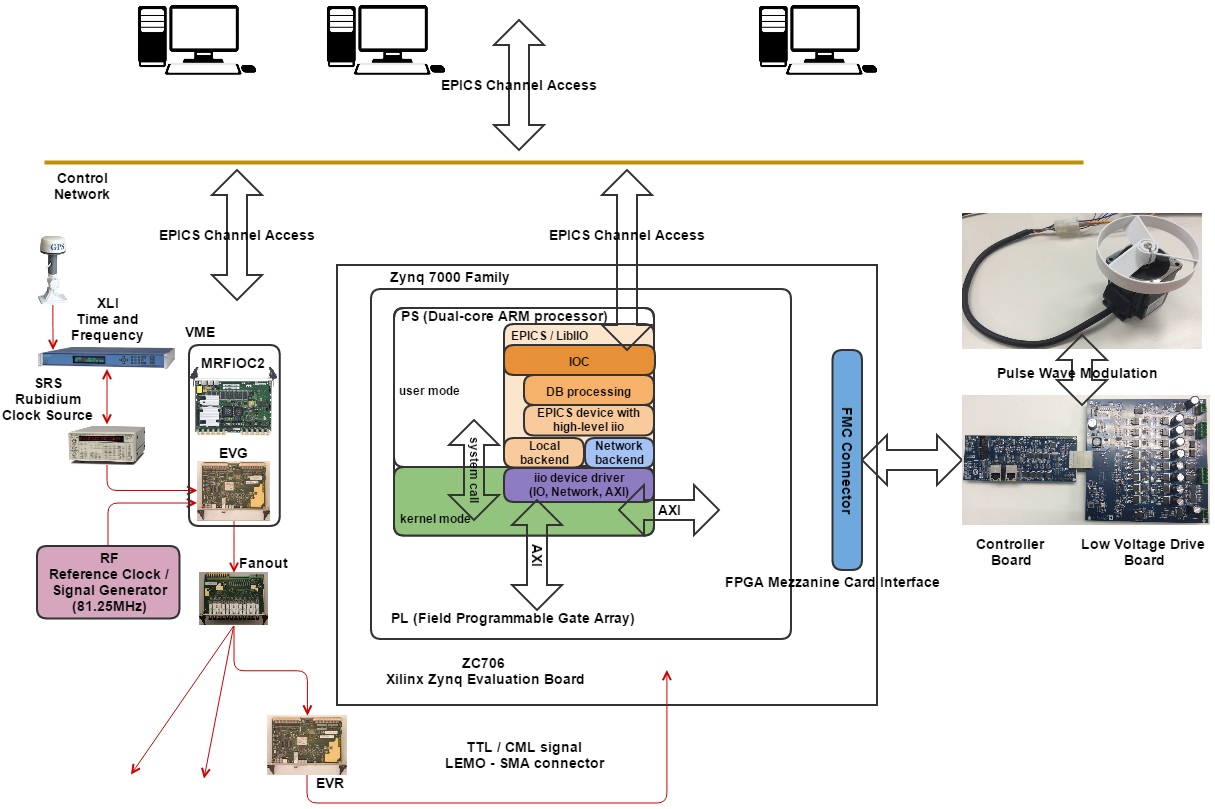
\includegraphics[width=1\textwidth]{./images/WEPGF124f3.eps}
		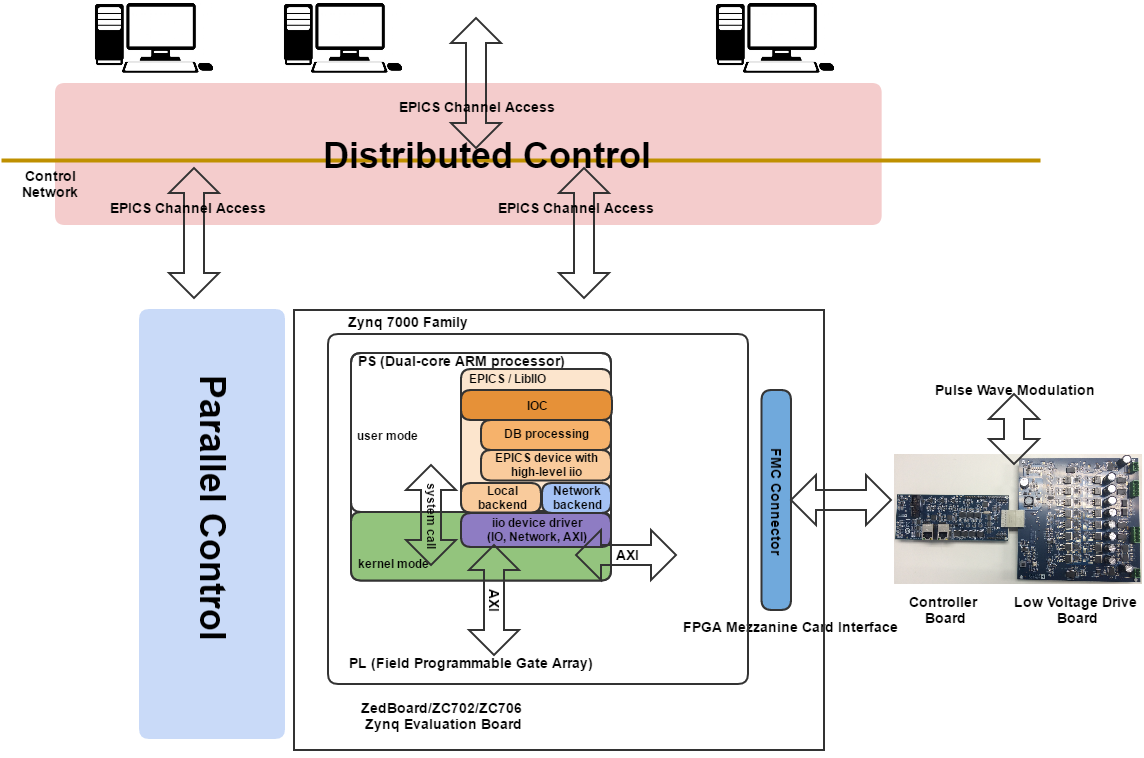
\includegraphics[width=25cm,height=23cm]{./images/img01.png}
	\end{figure}
\begin{itemize}
  	\item Distributed Control Environment
  	\begin{itemize}
	  	\item Linux OS on Zynq PS (ARM Processor)
  	  	\begin{itemize}
	  		\item ARM Cross Compile Tool Chain (arm-linuxgnueabihf)
	  		\item Linux Kernel Source (Linaro)\cite{linaro}
	  		\item Bootloader (BOOT.BIN: FSBL.elf, U-Boot.elf, uImage, Zynq.bif, User.bit) \cite{u-boot}
	  		\item Board Support Package (Linux Device Tree)
	  		\item Root File System (Busybox)\cite{busybox}
	  	\end{itemize}  	
  		\item Linux Device Driver : Interface between PS and PL is through the AXI of AMBA
  		\item EPICS Framework \cite{epics}
  		\begin{itemize}
	  		\item  Base R3.14.15.2
			\item  Control System Studio (CSS)	
		\end{itemize}  		  	  		
  		\item Libiio Library of Analog Device\cite{analog,iio}
	\end{itemize}  	
   	\item Parallel Processing Control Envrionment (ZC706)
  	\begin{itemize}
	  	\item Zynq PL (FPGA)
	  	\item FPGA VerilogHDL by Vivado (Used the HDL code of Analog Devices)
		\item Controller and Low Voltage Drive Board of Analog Devices
		\item Controller communicates with ZC706 via FMC Connector
		\item FMC Connection: XADC, Digital I/O, 2xGB Ethernet
		\item XADC and digital I/O signals to LVDB
		\item PWM Signal Generation through MOSFET Gate Drivers
		\item External Power: 12 $\sim$24 DC to LVDB	  			  		
  	\end{itemize}
\end{itemize}
\end{mdframed}

\subsection*{Software Defined System on Chip (SDSoC) Environment}
\vspace{2mm}
\begin{mdframed}[roundcorner=10pt]
\begin{figure}[H]
\centering
  %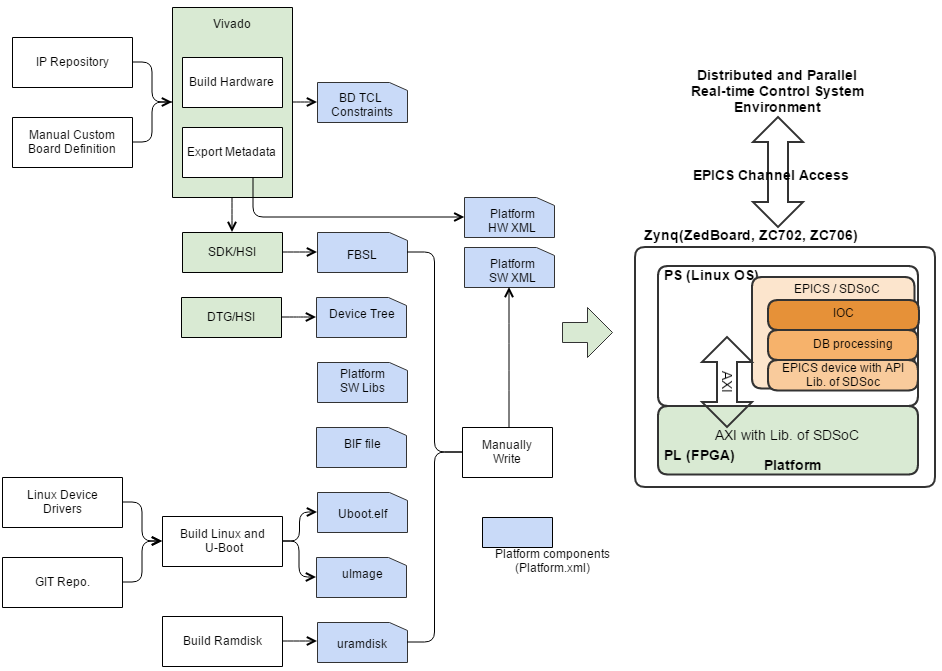
\includegraphics[width=.9\columnwidth]{./images/img03.png}
  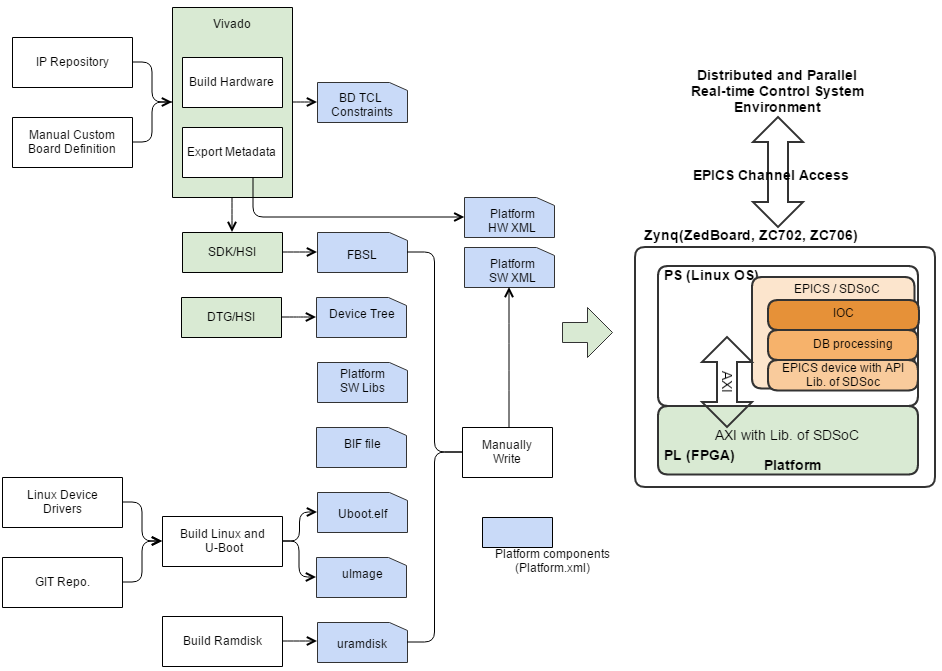
\includegraphics[width=25cm,height=20cm]{./images/img03.png}
%\caption{The timing system prototyping}
\label{fig:timing_prototype}
\end{figure}
The SDSoC\cite{sdsoc} environment is an Eclipse-based Integrated Development Environment (IDE) for implementing embedded systems using the zynq programmable SoC platform. The SDSoC environment includes support for the ZC702, ZC706, MicroZed, ZedBoard and Zybo development boards featuring the Zynq-7000 AP SoC.

Using SDSoC platform can implement as follows:
\begin{itemize}
\item Hardware and Software Architecture
\item Application Context including Linux OS
\item Bootloader
\item Root File System
\item High Level Libraries and Applications for Interface with PL
\end{itemize}

In addition, EPICS Framework on Linux Built using SDSoC :
\begin{itemize}
\item EPICS Base R3.14.15.2
\item EPICS Device Suport Routine with High Level Library Interface which developed and deployed with SDSoC
\end{itemize}
\end{mdframed}

\section*{\centering Future Plan}
\vspace{2mm}
\begin{mdframed}[roundcorner=10pt]
In order to connect the distributed processing system and parallel processing system more effectively, it should provide a unified interface layer for the specific various parallel processing hardwares. For the purpose of developing the unified parallel processing interface layer it can be used Open Computer Lanaguage (OpenCL)\cite{opencl}.

\begin{figure}[H]
	\centering
	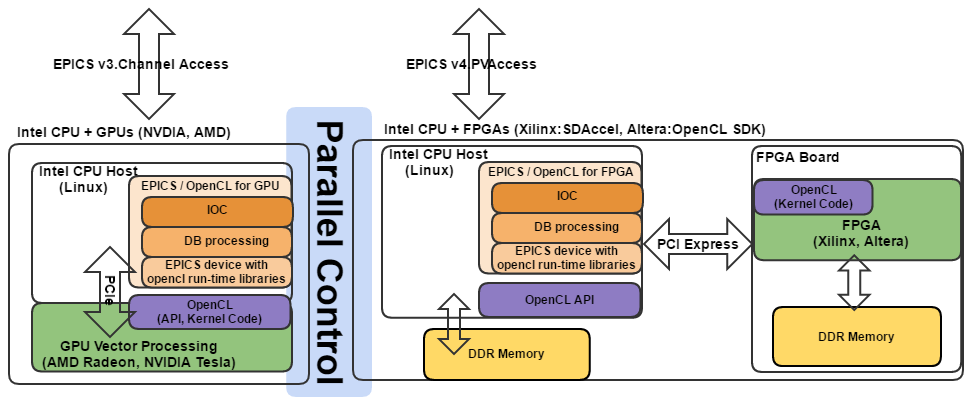
\includegraphics[width=25cm,height=13cm]{./images/img02.png}
\end{figure}

OpenCL\cite{opencl_wiki,opencl_on_altera} is a framework or programming model for writing programs that execute across heterogeneous platforms consisting of CPUs, GPUs, DSPs, FPGAs and other processors or hardware accelerators and was developed by the Khronos group.
\begin{itemize}
\item Hardwares Support for OpenCL for Parallel Control Environment
	\begin{itemize}
		\item  GPU: AMD Radeon or NVIDIA GeForce
		\item  FPGA: Xilinx - SDAccel or Altera - OpenCL SDK
	\end{itemize}  			
\item Abstract layer using OpenCL for Parallel Processing
\begin{itemize}
	\item  OpenCL (1.2 or 2.0)
	\item  Host Code: OpenCL API-Serial, Sequence code
	\item  Kernel Code: Parallel Code for GPUs, FPGAs
	\item  EPICS Device Support IOC code + Host Code	
\end{itemize}  			
\end{itemize}
Adopting EPICS v4, it will be interfaced large amounts of data and complex data to be processed in the parallel processing of a variety of experimental devices.
\begin{itemize}
\item EPICS Version 4\cite{epics_v4} for Distributed Control Environment
	\begin{itemize}
		\item  Normative Types - Collection of Structured Data Types \cite{epics_v4_normative}
		\item  pvCommon, pvData, pvAccess, pvaSrv Modules	
	\end{itemize}  			
\end{itemize}
\end{mdframed}

\columnbreak

\section*{\centering Conclusion}
\vspace{2mm}
\begin{mdframed}[roundcorner=10pt]
Big scientific experiment facilities such as accelerators, nuclear fusion, and telescope are  required by the unity of the heterogenous distributed control system and the fast response according to its characteristic. These requirements for \textbf{\textit{\underline{the distributed and parallel environments}}} must be satisfied at the same time. If the distributed control system using EPICS makes a connection with the high speed parallel processing of FPGA, it is possible to improve the performance and efficiency of the control system. \textbf{\textit{\underline{Zynq SoC}}} can be considered as an ideal device to satisfy with \textbf{\textit{\underline{the distributed and high-speed parallel control system}}} at the same time. More and more, the control environment of devices used in the big science experiment of the future will be used the distributed processing environment combined with the parallel processing environment. Therefore, it expect to be increased the requirements for the unified software abstraction layer to operate the heterogenous parallel proccessing hardwares."FPGA-based heterogeneous system (CPU + FPGA) using the OpenCL standard has a significant time-to-market advantage compared to traditional FPGA development using lower level hardware description languages (HDLs) such as Verilog or VHDL"\cite{opencl_on_altera}.  As a result, utilizing the \textbf{\textit{\underline{OpenCL standard}}} on the heterogeneous parallel processing hardwares may offer significantly \textbf{\textit{\underline{higher performance}}} and \textbf{\textit{\underline{the unified abastract layer}}} at much lower power. 
\end{mdframed}

\section*{\centering Acknowledgement}
\vspace{2mm}
This work is supported by the Rare Isotope Science Project funded by Ministry of Science, ICT and Future Planning \textbf{(MSIP)} and National Research Foundation \textbf{(NRF)} of KOREA.

\begin{thebibliography}{13}   % Use for  1-9  references
%\begin{thebibliography}{99} % Use for 10-99 references

\bibitem{risp} Y.~K.~Kwon, {\it et. al},``Status of Rare Isotope Science Project in Korea'',
Few-Body Syst 54, 961-966, (2013).

\bibitem{linaro}
Linaro Document website, https://en.wikipedia.org/wiki/Linaro

\bibitem{u-boot}
U-Boot Document website, http://www.denx.de/wiki/U-Boot

\bibitem{busybox}
Busybox Document website, http://www.busybox.net/

\bibitem{epics}
EPICS website, http://www.aps.anl.gov/epics/

\bibitem{analog}
Analog Devices website, http://www.analog.com

\bibitem{iio}
Industrial I/O Document website, \\ https://wiki.analog.com/resources/tools-software/linux-software/libiio

\bibitem{sdsoc}
SDSoC Document,\\ http://www.xilinx.com/support/documentation/sw\_manuals/xilinx2016\_1/ug1146-sdsoc-platforms-and-libraries.pdf

\bibitem{opencl}
OpenCL, https://www.khronos.org/opencl/

\bibitem{opencl_wiki}
OpenCL Definition, https://en.wikipedia.org/wiki/OpenCL

\bibitem{opencl_on_altera}
OpenCL on Altera, https://www.altera.com/en\_US/pdfs/literature/wp/wp-01173-opencl.pdf

\bibitem{epics_v4}
EPICS Version 4, http://epics-pvdata.sourceforge.net/

\bibitem{epics_v4_normative}
EPICS Version 4 Normative Types,\\ http://epics-pvdata.sourceforge.net/docbuild/normativeTypesCPP/tip/\\documentation/ntCPP.html

\end{thebibliography}
\end{multicols}

%\vspace{13mm}

%\begin{minipage}[b]{1\linewidth}

%\section*{RAON Major Operations Modes}
%\vspace{2mm}
%\begin{figure}[H]
 % \includegraphics[width=0.99\columnwidth]{./images/raon_all_modes.eps}
%\end{figure}

%\end{minipage}

\end{document}

